\documentclass[journal,12pt,twocolumn]{IEEEtran}
\usepackage{setspace}
\usepackage{gensymb}
\usepackage{bm}
\usepackage{caption}
%\usepackage{multirow}
%\usepackage{multicolumn}
%\usepackage{subcaption}
%\doublespacing
\singlespacing
\usepackage{csvsimple}
\usepackage{amsmath}
\usepackage{multicol}
%\usepackage{enumerate}
\usepackage{amssymb}
%\usepackage{graphicx}
\usepackage{newfloat}
%\usepackage{syntax}
\usepackage{listings}
\usepackage{iithtlc}
\usepackage{color}
\usepackage{tikz}
\usetikzlibrary{shapes,arrows}



%\usepackage{graphicx}
%\usepackage{amssymb}
%\usepackage{relsize}
%\usepackage[cmex10]{amsmath}
%\usepackage{mathtools}
%\usepackage{amsthm}
%\interdisplaylinepenalty=2500
%\savesymbol{iint}
%\usepackage{txfonts}
%\restoresymbol{TXF}{iint}
%\usepackage{wasysym}
\usepackage{amsthm}
\usepackage{mathrsfs}
\usepackage{txfonts}
\usepackage{stfloats}
\usepackage{cite}
\usepackage{cases}
\usepackage{mathtools}
\usepackage{caption}
\usepackage{enumerate}	
\usepackage{enumitem}
\usepackage{amsmath}
%\usepackage{xtab}
\usepackage{longtable}
\usepackage{multirow}
%\usepackage{algorithm}
%\usepackage{algpseudocode}
\usepackage{enumitem}
\usepackage{mathtools}
\usepackage{hyperref}
%\usepackage[framemethod=tikz]{mdframed}
\usepackage{listings}
    %\usepackage[latin1]{inputenc}                                 %%
    \usepackage{color}                                            %%
    \usepackage{array}                                            %%
    \usepackage{longtable}                                        %%
    \usepackage{calc}                                             %%
    \usepackage{multirow}                                         %%
    \usepackage{hhline}                                           %%
    \usepackage{ifthen}                                           %%
  %optionally (for landscape tables embedded in another document): %%
    \usepackage{lscape}     


\usepackage{url}
\def\UrlBreaks{\do\/\do-}


%\usepackage{stmaryrd}


%\usepackage{wasysym}
%\newcounter{MYtempeqncnt}
\DeclareMathOperator*{\Res}{Res}
%\renewcommand{\baselinestretch}{2}
\renewcommand\thesection{\arabic{section}}
\renewcommand\thesubsection{\thesection.\arabic{subsection}}
\renewcommand\thesubsubsection{\thesubsection.\arabic{subsubsection}}

\renewcommand\thesectiondis{\arabic{section}}
\renewcommand\thesubsectiondis{\thesectiondis.\arabic{subsection}}
\renewcommand\thesubsubsectiondis{\thesubsectiondis.\arabic{subsubsection}}

% correct bad hyphenation here
\hyphenation{op-tical net-works semi-conduc-tor}

%\lstset{
%language=C,
%frame=single, 
%breaklines=true
%}

%\lstset{
	%%basicstyle=\small\ttfamily\bfseries,
	%%numberstyle=\small\ttfamily,
	%language=Octave,
	%backgroundcolor=\color{white},
	%%frame=single,
	%%keywordstyle=\bfseries,
	%%breaklines=true,
	%%showstringspaces=false,
	%%xleftmargin=-10mm,
	%%aboveskip=-1mm,
	%%belowskip=0mm
%}

%\surroundwithmdframed[width=\columnwidth]{lstlisting}
\def\inputGnumericTable{}                                 %%
\lstset{
%language=C,
frame=single, 
breaklines=true,
columns=fullflexible
}
 

\begin{document}
%
\tikzstyle{block} = [rectangle, draw,
    text width=3em, text centered, minimum height=3em]
\tikzstyle{sum} = [draw, circle, node distance=3cm]
\tikzstyle{input} = [coordinate]
\tikzstyle{output} = [coordinate]
\tikzstyle{pinstyle} = [pin edge={to-,thin,black}]

\theoremstyle{definition}
\newtheorem{theorem}{Theorem}[section]
\newtheorem{problem}{Problem}
\newtheorem{proposition}{Proposition}[section]
\newtheorem{lemma}{Lemma}[section]
\newtheorem{corollary}[theorem]{Corollary}
\newtheorem{example}{Example}[section]
\newtheorem{definition}{Definition}[section]
%\newtheorem{algorithm}{Algorithm}[section]
%\newtheorem{cor}{Corollary}
\newcommand{\BEQA}{\begin{eqnarray}}
\newcommand{\EEQA}{\end{eqnarray}}
\newcommand{\define}{\stackrel{\triangle}{=}}

\bibliographystyle{IEEEtran}
%\bibliographystyle{ieeetr}

\providecommand{\nCr}[2]{\,^{#1}C_{#2}} % nCr
\providecommand{\nPr}[2]{\,^{#1}P_{#2}} % nPr
\providecommand{\mbf}{\mathbf}
\providecommand{\pr}[1]{\ensuremath{\Pr\left(#1\right)}}
\providecommand{\qfunc}[1]{\ensuremath{Q\left(#1\right)}}
\providecommand{\sbrak}[1]{\ensuremath{{}\left[#1\right]}}
\providecommand{\lsbrak}[1]{\ensuremath{{}\left[#1\right.}}
\providecommand{\rsbrak}[1]{\ensuremath{{}\left.#1\right]}}
\providecommand{\brak}[1]{\ensuremath{\left(#1\right)}}
\providecommand{\lbrak}[1]{\ensuremath{\left(#1\right.}}
\providecommand{\rbrak}[1]{\ensuremath{\left.#1\right)}}
\providecommand{\cbrak}[1]{\ensuremath{\left\{#1\right\}}}
\providecommand{\lcbrak}[1]{\ensuremath{\left\{#1\right.}}
\providecommand{\rcbrak}[1]{\ensuremath{\left.#1\right\}}}
\theoremstyle{remark}
\newtheorem{rem}{Remark}
\newcommand{\sgn}{\mathop{\mathrm{sgn}}}
\providecommand{\abs}[1]{\left\vert#1\right\vert}
\providecommand{\res}[1]{\Res\displaylimits_{#1}} 
\providecommand{\norm}[1]{\lVert#1\rVert}
\providecommand{\mtx}[1]{\mathbf{#1}}
\providecommand{\mean}[1]{E\left[ #1 \right]}
\providecommand{\fourier}{\overset{\mathcal{F}}{ \rightleftharpoons}}
\providecommand{\gauss}[2]{\mathcal{N}\ensuremath{\left(#1,#2\right)}}
%\providecommand{\hilbert}{\overset{\mathcal{H}}{ \rightleftharpoons}}
\providecommand{\system}{\overset{\mathcal{H}}{ \longleftrightarrow}}
	%\newcommand{\solution}[2]{\textbf{Solution:}{#1}}
\newcommand{\solution}{\noindent \textbf{Solution: }}
\newcommand{\myvec}[1]{\ensuremath{\begin{pmatrix}#1\end{pmatrix}}}
\providecommand{\dec}[2]{\ensuremath{\overset{#1}{\underset{#2}{\gtrless}}}}
\DeclarePairedDelimiter{\ceil}{\lceil}{\rceil}
%\numberwithin{equation}{subsection}
\numberwithin{equation}{section}
%\numberwithin{problem}{subsection}
%\numberwithin{definition}{subsection}
\makeatletter
\@addtoreset{figure}{section}
\makeatother

\let\StandardTheFigure\thefigure
%\renewcommand{\thefigure}{\theproblem.\arabic{figure}}
\renewcommand{\thefigure}{\thesection}


%\numberwithin{figure}{subsection}

%\numberwithin{equation}{subsection}
%\numberwithin{equation}{section}
%\numberwithin{equation}{problem}
%\numberwithin{problem}{subsection}
\numberwithin{problem}{section}
%%\numberwithin{definition}{subsection}
%\makeatletter
%\@addtoreset{figure}{problem}
%\makeatother
\makeatletter
\@addtoreset{table}{section}
\makeatother

\let\StandardTheFigure\thefigure
\let\StandardTheTable\thetable
\let\vec\mathbf
%%\renewcommand{\thefigure}{\theproblem.\arabic{figure}}
%\renewcommand{\thefigure}{\theproblem}

%%\numberwithin{figure}{section}

%%\numberwithin{figure}{subsection}



\def\putbox#1#2#3{\makebox[0in][l]{\makebox[#1][l]{}\raisebox{\baselineskip}[0in][0in]{\raisebox{#2}[0in][0in]{#3}}}}
     \def\rightbox#1{\makebox[0in][r]{#1}}
     \def\centbox#1{\makebox[0in]{#1}}
     \def\topbox#1{\raisebox{-\baselineskip}[0in][0in]{#1}}
     \def\midbox#1{\raisebox{-0.5\baselineskip}[0in][0in]{#1}}

\vspace{3cm}



\title{ 
	\logo{
Linear Classification
	}
}

\author{ G V V Sharma$^{*}$% <-this % stops a space
	\thanks{*The author is with the Department
		of Electrical Engineering, Indian Institute of Technology, Hyderabad
		502285 India e-mail:  gadepall@iith.ac.in. All content in this manual is released under GNU GPL.  Free and open source.}
	
}	

\maketitle

\tableofcontents

\bigskip

\renewcommand{\thefigure}{\theenumi}
\renewcommand{\thetable}{\theenumi}


\begin{abstract}
	
This manual provides an introduction to linear lethods in regression.
\end{abstract}

\section{The Gaussian Distribution}
\begin{enumerate}[label=\thesection.\arabic*
,ref=\thesection.\theenumi]

\item
\label{ch1_prob1}
Generate a Gaussian random number with 0 mean and unit variance.

%
\solution Open a text editor and type the following program.

%%
\lstinputlisting{./codes/1.1.py}
%%
Save the file as gaussian\_no.py and run the program.
%
\item
The mean of a random variable $X$ is defined as
%
\begin{equation}
E\sbrak{X} = \frac{1}{N}\sum_{i=1}^{N}X_i
\end{equation}
%
and its variance as
%
\begin{equation}
\text{var}\sbrak{X} = E\sbrak{X- E\sbrak{X}}^2 
\end{equation}
%
Verify that the program in \ref{ch1_prob1} actually generates a Gaussian random variable with 0 mean and unit variance.

\solution  Use the header in the previous program, type the following code and execute.
\lstinputlisting{./codes/1.2.py}
%
%
\item
Using the previous program, verify you results for different values of the mean and variance.

\end{enumerate}

\section{CDF and PDF}
\begin{enumerate}[label=\thesection.\arabic*
,ref=\thesection.\theenumi]

\item
A Gaussian random variable $X$ with mean 0 and unit variance can be expressed as $X \sim \mathcal{N}\brak{0,1}$. Its cumulative distribution function (CDF) is defined as
\begin{equation}
F_X(x) = \pr{X < x}, 
\end{equation}
Plot $F_X(x)$.

\solution  The following code yields Fig. \ref{ch1_prob3_fig}.
\lstinputlisting{./codes/1.3.py}
%
\begin{figure}
\centering
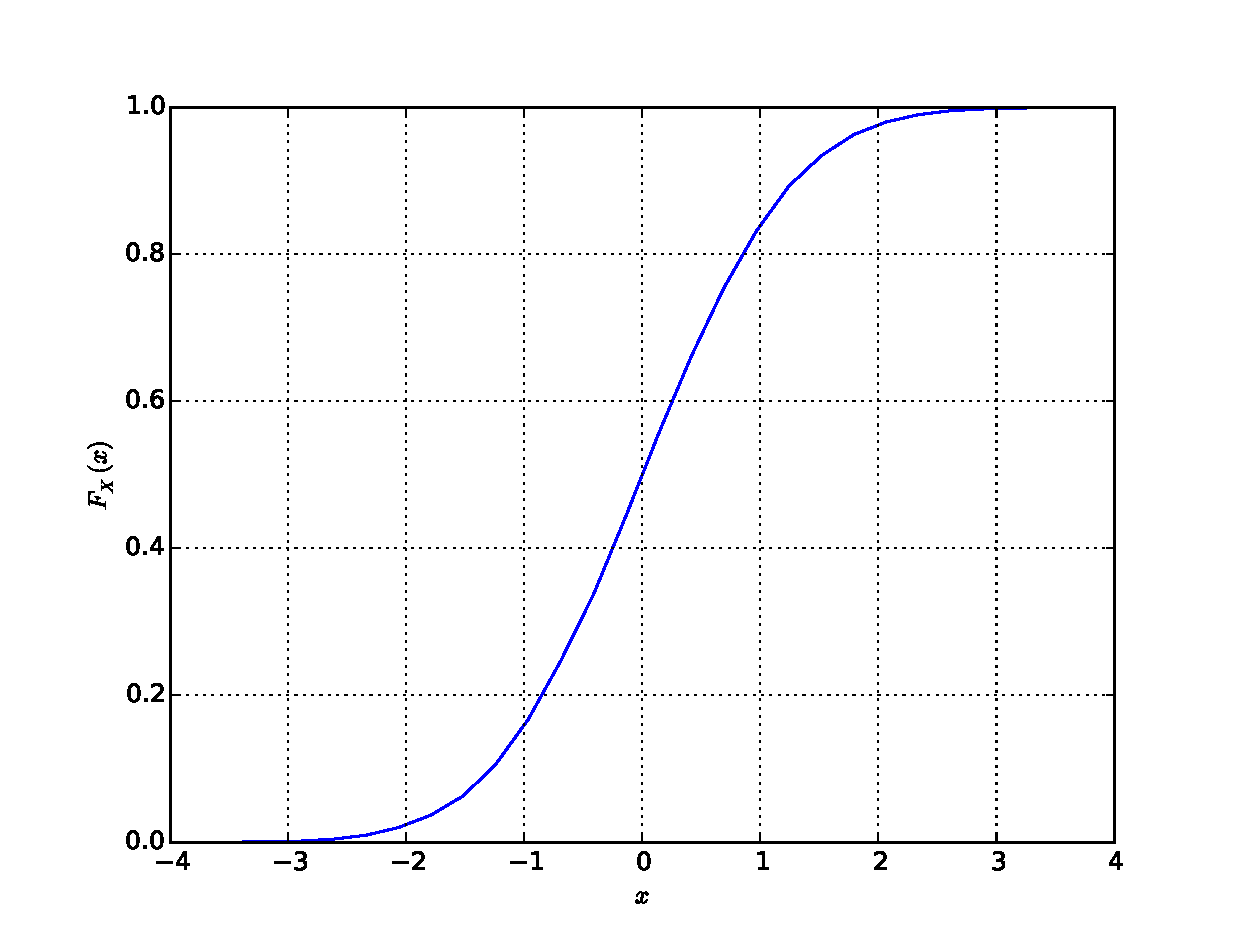
\includegraphics[width=\columnwidth]{./figs/ch1_prob3_fig}
\caption{CDF of $X$}
\label{ch1_prob3_fig}
\end{figure}
%
\item
List the properties of $F_X(x)$ based on Fig. \ref{ch1_prob3_fig}.

%
\item
Let
%
\begin{equation}
p_{X}(x_i) = \frac{F_{X}(x_i)-F_{X}(x_{i-1})}{h}, i = 1, 2, \dots
{h}
\end{equation}
%
for $x_i = x_{i-1}+h, x_1 = -4$. Plot $p_X(x_i)$.  On the same graph, plot
%
\begin{equation}
p_{X}(x) = \frac{1}{\sqrt{2\pi}}e^{-x^2/2}, - 4 < x < 4
\end{equation}
%

%
\solution The following code yields the graph in Fig. \ref{ch1_prob4_fig}
\begin{lstlisting}
https://github.com/gadepall/EE1390/raw/master/manuals/supervised/linear_class/codes/1.4.py
\end{lstlisting}
\begin{figure}
\centering
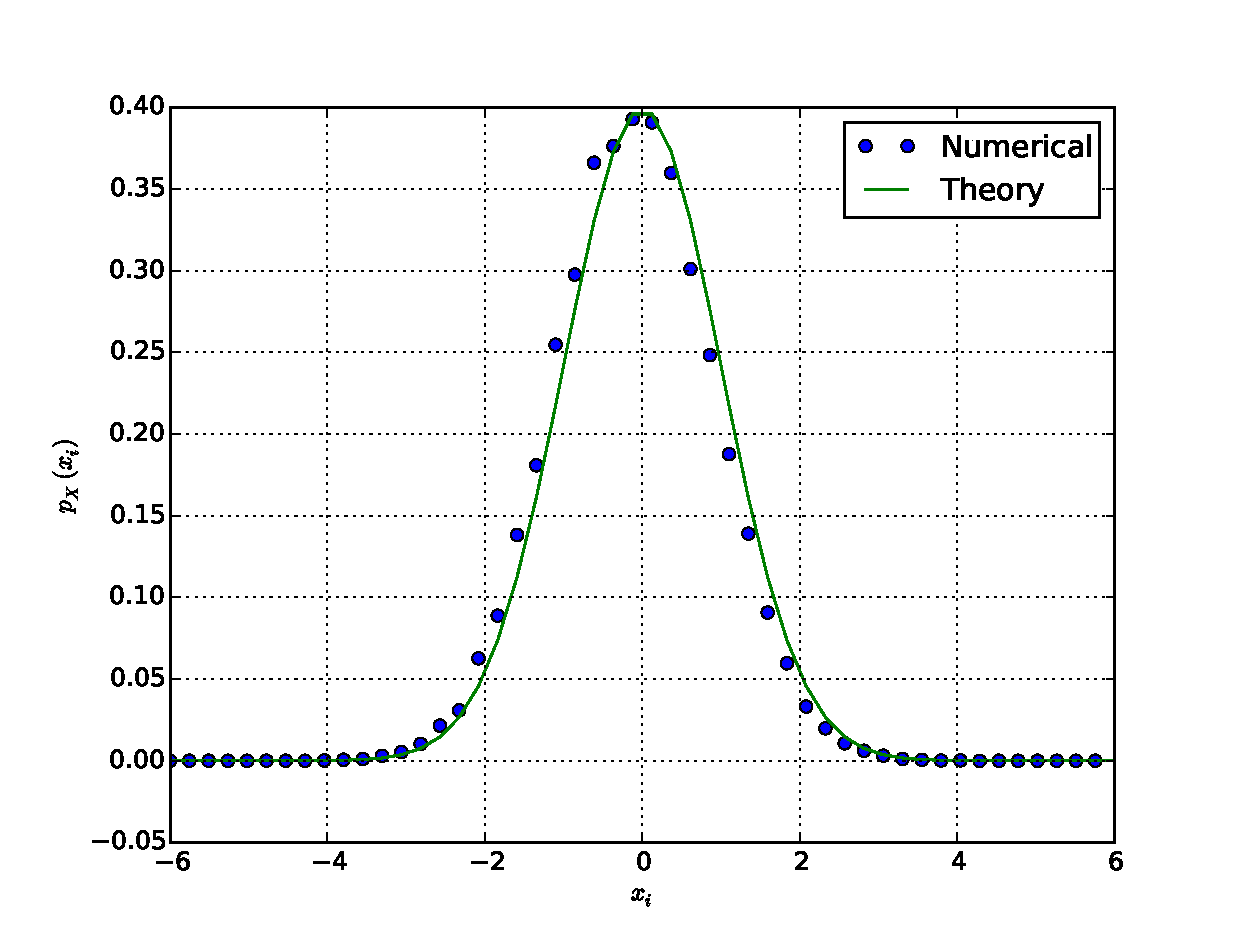
\includegraphics[width=\columnwidth]{./figs/ch1_prob4_fig}
\caption{The PDF of $X$}
\label{ch1_prob4_fig}
\end{figure}
%
Thus, the PDF is the derivative of the CDF.  For $X\sim \mathcal{N}\brak{0,1}$, the PDF is
%
\begin{equation}
p_{X}(x) = \frac{1}{\sqrt{2\pi}}e^{-\frac{x^2}{2}}, \quad -\infty < x < \infty
\end{equation}
\item
%
For $X\sim \mathcal{N}\brak{\mu,\sigma^2}$,
\begin{equation}
p_{X}(x) = \frac{1}{\sqrt{2\pi}\sigma}e^{-\frac{\brak{x-\mu}^2}{2\sigma^2}}, \quad -\infty < x < \infty
\end{equation}
Plot $p_{X}(x)$ for different values of $\mu$ and $\sigma$ in the same graph.  Comment.
%
\end{enumerate}

\section{Detection \& Estimation}
\begin{enumerate}[label=\thesection.\arabic*
,ref=\thesection.\theenumi]
%\item
%Let $Y \in \cbrak{1,-1}$.  Generate $S$ such that the numbers 1 and -1 appear with equal probability.  This is 
%a random variable formulation of the coin tossing experiment.
%
%\solution  The following script generates the numbers 1 and -1 with 
%equal probability.
%\lstinputlisting{./codes/2.1.py}
%%
%\item
%Verify that the script in the previous problem generates equiprobable symbols.

%\item
%Suppose $S \in \cbrak{1,-1}$ and 
%%
%\begin{equation}
%X = AS + N
%\end{equation}
%%
%where $N \sim \gauss{0}{1}$ and $A = 4$.  Obtain a scatterplot of  $\brak{X,0}$.
%
%\solution 
\item Use the following code 
%%Fig. \ref{ch2_bpsk_sim}
%\lstinputlisting{./codes/2.3.py}
\begin{lstlisting}
https://raw.githubusercontent.com/gadepall/EE1390/master/manuals/supervised/linear_class/codes/2.3.py
\end{lstlisting}
%
to generate  a scatterplot of $X$.
%%
%\begin{figure}
%\centering
%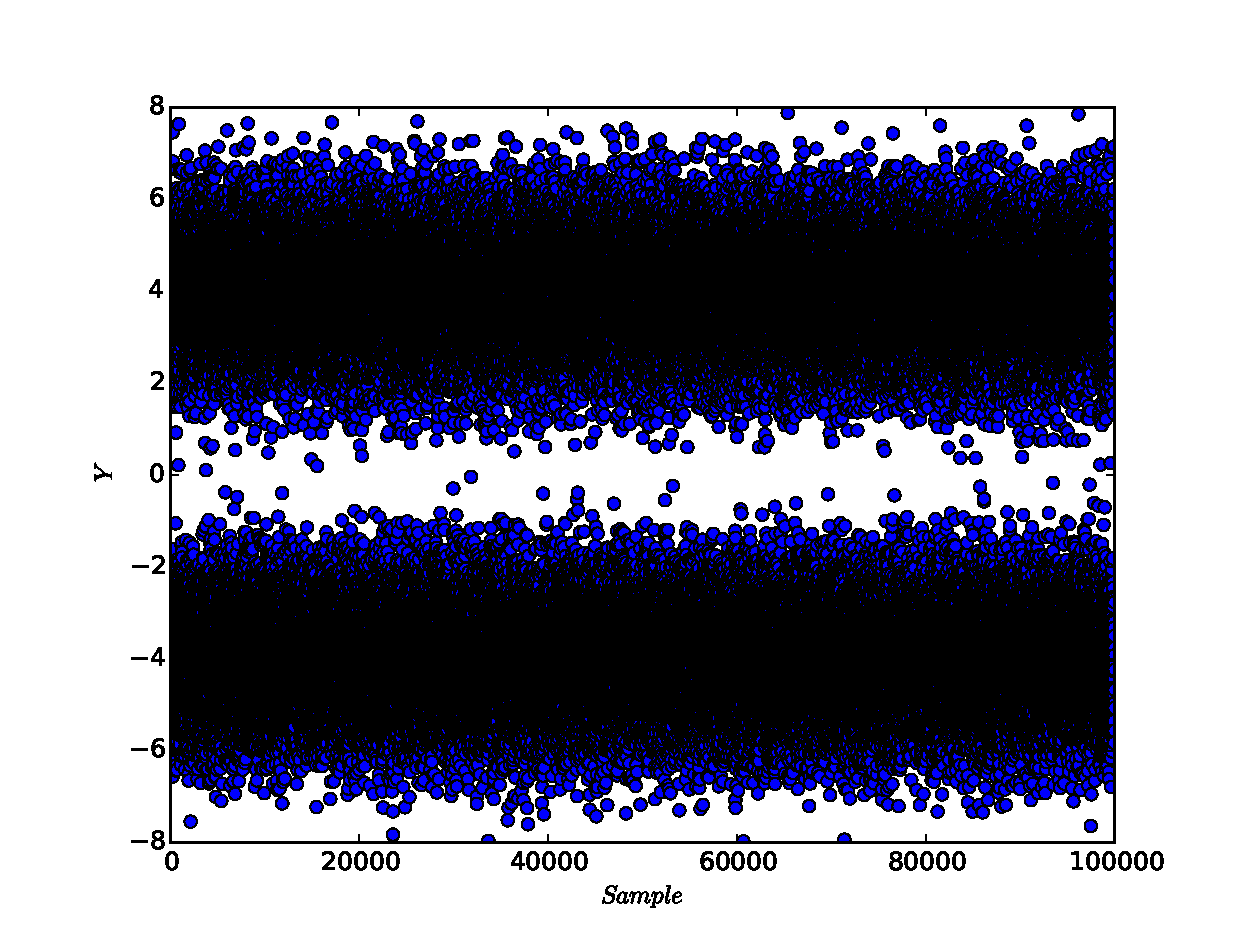
\includegraphics[width=\columnwidth]{./figs/ch2_bpsk_sim}
%\caption{Plot of $Y$}
%\label{ch2_bpsk_sim}
%\end{figure}
%
\item Suppose you wanted to classify  $X$ into two groups.  How would you do so by looking at the scatterplot?
%$Y$ is 1 or -1.
%

\end{enumerate}

%
\section{Bayes Classifier}
\begin{enumerate}[label=\thesection.\arabic*
,ref=\thesection.\theenumi]
%
\item Let
%
\begin{align}
x = A\brak{2s-1} + n
\end{align}
%
where $s \in \cbrak{0,1}, n \sim \gauss{0}{1}$.

\item Show that
\begin{align}
x|0  &\sim \gauss{-A}{1}
\\
x|1 &\sim \gauss{A}{1}
\end{align}
%plot $p_{X}(X=x|G=0)$ and   $p_{X}(X=x|G=1)$ for $A = 4$.
\solution From the given information, for $s=0$,
\begin{align}
x|0  &= -A + n
\\
\implies \mean{x|0}  &= -A 
\\
\text{and } \mean{\brak{x+A}^2|0}  &= \mean{n^2} = 1 
\end{align}
%
Similar approach can be used for  $x|1$.
\item Find
\begin{equation}
p_{X|0}(x)\text{ and } p_{X|1}(x)
\end{equation}
\solution
\begin{align}
p_{X}(x|0)  &= \frac{1}{\sqrt{2\pi}}e^{-\frac{\brak{x+A}^2}{2}}, 
\quad 
-\infty < x < \infty
\\
p_{X}(x|1)  &= 
\frac{1}{\sqrt{2\pi}}e^{-\frac{\brak{x-A}^2}{2}}, \quad 
-\infty < x < \infty
\end{align}
\item Show that $e^{-x}$ is monotonically decreasing.
\item Find
\begin{equation}
p_{X}(x|1) \dec{1}{0} p_{X}(x|0)
\end{equation}
%
\solution The given condition can be expressed as
\begin{align}
 \frac{1}{\sqrt{2\pi}}e^{-\frac{\brak{x-A}^2}{2}}
&\dec{1}{0}
\frac{1}{\sqrt{2\pi}}e^{-\frac{\brak{x+A}^2}{2}}
\\
\implies -\frac{\brak{x-A}^2}{2}
&\dec{1}{0}
-\frac{\brak{x+A}^2}{2}
\\
\implies x &\dec{1}{0} 0
\end{align}
%
after simplification.
\item Show that 
\begin{align}
p_{X}(0|x) \dec{0}{1} p_{X}(1|x)
\\
\implies p_{X}(x|0) \dec{0}{1} p_{X}(x|1)
\end{align}
if
\begin{equation}
p(0)=p(1)
\end{equation}
%
\solution Since 
\begin{align}
p_{X}(1|x) \dec{1}{0} p_{X}(0|x)
\\
\implies \frac{p_{X}(x|1) p(1)}{p(x)}\dec{1}{0} 
\frac{p_{X}(x|0)p(0)}{p(x)},
\end{align}
%
the result follows.
\end{enumerate}
\section{Probability of Error}
\begin{enumerate}[label=\thesection.\arabic*
,ref=\thesection.\theenumi]
\item
Suppose $S=1$ and $Y$ is what you detected.  Find $\pr{\hat{Y}=-1/S=1}$.

%
\item
Plot  $\pr{Y=-1|S=1}$ with respect to $A$.

%
\item
For $X \sim \mathcal{N}\brak{0,1}$, the $Q$-function is defined as
\begin{equation}
Q(x) = \pr{X > x}, \quad x > 0
\end{equation}
Express $\pr{Y=-1|S=1}$ in terms of the $Q$-function. Plot this expression with respect to $A$ 
from 0 to 10 dB and compare with the result obtained through simulation.


\item
Now consider a threshold $\lambda > 0$ and find the average probability of error. Plot this with respect to $\lambda$.

%
\item
From the graph in the previous problem, find the optimum threshold so that the probability of error is minimum.
\item
The signal to noise ratio of the above system is defined as 
\begin{equation}
SNR = \frac{A^2}{\mean{N^2}}
\end{equation}

\end{enumerate}



\section{Linear Discriminant Analysis}
\begin{enumerate}[label=\thesection.\arabic*
,ref=\thesection.\theenumi]
\item The multivariate Gaussian distribution is defined as
%
\begin{multline}
p_{\vec{x}}\brak{\vec{x}}
\\
=\frac{1}{\sqrt{\brak{2\pi}^k\abs{\bm{\Sigma}}}}\exp\cbrak{-\frac{1}{2}\brak{\vec{x}-\bm{\mu}}^T\bm{\Sigma}^{-1}\brak{\vec{x}-\vec{\mu}}}
\end{multline}
%
where $\bm{\mu}$ is the mean vector, $\bm{\Sigma} = E\sbrak{\brak{\vec{x}-\bm{\mu}}\brak{\vec{x}-\bm{\mu}}^T}$ is the covariance matrix and $\abs{\bm{\Sigma}}$ is the determinant of $\bm{\Sigma}$.
\item For
\begin{align}
\vec{x} = \myvec{x_1\\x_2},
\end{align}
show that
{\small
\begin{multline}
p_{\vec{x}}\brak{\vec{x}}= \frac{1}{2\pi 
\sigma_{1}\sigma_2\sqrt{1-\rho^2}}\exp\lsbrak{-\frac{1}{2\brak{1-\rho^2}}}
\\
\times 
\rsbrak{\cbrak{\frac{\brak{x_1-\mu_1}^2}{\sigma_1^2}+\frac{\brak{x_2-\mu_2}^2}{\sigma_2^2}-\frac{2\rho\brak{x_1-\mu_1}\brak{x_2-\mu_2}}{\sigma_1\sigma_2}}}
\end{multline}
}
%
where
%
\begin{align}
\bm{\mu}=
\begin{pmatrix*}
\mu_1 \\
\mu_2
\end{pmatrix*},
\bm{\Sigma} = 
\begin{pmatrix*}%[r]
\sigma_1^2 & \rho\sigma_1\sigma_2 \\
\rho\sigma_1\sigma_2 & \sigma_2^2
\end{pmatrix*}
\end{align}
%
\item Let
%
\begin{align}
\vec{s}_0=\myvec{a\\0}
\\
\vec{s}_1=\myvec{0\\a}
\end{align}
If 
\begin{align}
\vec{x} = \vec{s} + \vec{n}
\end{align}
%
where $\vec{s}\in \cbrak{\vec{s}_0,\vec{s}_1}$ and $\vec{n}\sim \mathcal{N}\brak{0,\sigma^2 \vec{I}}$, show 
that
\begin{align}
\mathbf{x}|0 = 
\begin{pmatrix*}
a + n_{1}\\
n_{2}
\end{pmatrix*},
\end{align}
and 
\begin{align}
\mathbf{x}|1 = 
\begin{pmatrix*}
n_{1}\\
a + n_{2}
\end{pmatrix*},
\end{align}
%
\item Find
\begin{align}
\label{eq:least_vecs}
p_{\vec{x}|\vec{s}_0}(\vec{x})
\\
p_{\vec{x}|\vec{s}_1}(\vec{x})
\end{align}
%
\item How will you decide between $\vec{s}_0$ and $\vec{s}_1$ if you have $\vec{x}$?
%
%
%\item A Gaussian random variable $X\sim\gauss{\mu}{\sigma^2}$ has the pdf
%
%\begin{equation}
%p_{X}(x) = \frac{1}{\sqrt{2\pi}\sigma}e^{-\brak{x-\mu}^2/2\sigma^2} - \infty < x < \infty
%\end{equation}
%
\end{enumerate}
\section{Optimum Classifier}
\begin{enumerate}[label=\thesection.\arabic*
,ref=\thesection.\theenumi]

\item Let $\brak{\vec{X},\vec{G}}$ be an input/output dataset, whose relation $f$ is unknown. Also
\begin{align}
\vec{g}\in\vec{G} = \cbrak{\vec{g}_k}_{k=1}^{K}
%\\
%\hat{\vec{G}} &= f\brak{\vec{X}}
\end{align}
Let 
\begin{align}
\label{eq:bayes_correct}
C\brak{\vec{g}_k,\vec{g}_l} =
\begin{cases}
1 & k= l
\\
0 & k\ne l
\end{cases}
\end{align}
%
where $\vec{g}_i$ are different classes of output data. Thus $C$ is a {\em correctness} metric.
\item Show that 
\begin{align}
\max_{\vec{g}\in\vec{G}}E\sbrak{C\brak{\vec{G},f\brak{\vec{X}}}} 
= \max_{\vec{g}\in\vec{G}}p\brak{\vec{g}|\vec{X}=\vec{x}} 
\end{align}
\solution In the above, 
\begin{multline}
\max_{\vec{g}\in\vec{G}}E\sbrak{C\brak{\vec{G},f\brak{\vec{X}}}} 
\\
= \max_{\vec{g}\in\vec{G}}E_\vec{X}\sbrak{E_{\vec{G}}\cbrak{C\brak{\vec{G},f\brak{\vec{x}}}}} 
\end{multline}
%
\begin{align}
&=\max_{\vec{g}\in\vec{G}}\sum_{k=1}^{K}C\cbrak{\vec{g}_k,\vec{g}}p\brak{\vec{g}_k|\vec{X}=\vec{x}} 
\end{align}
From \eqref{eq:bayes_correct}, the above expression simplifies to
\begin{align}
\max_{\vec{g}\in\vec{G}}E\sbrak{C\brak{\vec{G},f\brak{\vec{X}}}} =\max_{\vec{g}\in\vec{G}}p\brak{\vec{g}|\vec{X}=\vec{x}} 
\end{align}
%
\end{enumerate}

%\section{Quadratic Discriminant Analysis}
%\begin{enumerate}[label=\thesection.\arabic*
%,ref=\thesection.\theenumi]
%\item Find
%
%\end{enumerate}
%
\end{document}
%
%\section{Subset Selection}
%\begin{enumerate}[label=\thesection.\arabic*
%,ref=\thesection.\theenumi]
%\item Explain the best-subset selection method through an example.
%\item Explain the forward and backward subset selection method through an example.
%\item Explain the forward-stagewise  selection method through an example.
%\end{enumerate}
%\section{Introduction}
%\begin{enumerate}[label=\thesection.\arabic*
%,ref=\thesection.\theenumi]
%\item Let 
%%
%\begin{align}
%\vec{X}^T\brak{\vec{y}-\vec{X}\vec{w}} &= 0
%\\
%\hat{\vec{w}} &= \brak{\vec{X}^T\vec{X}}^{-1}\vec{X}^T \vec{y}
%\end{align}
%%
%where $\vec{w}$ is $p \times 1$ and $\vec{X}$ is $N \times p$.  Show that
%\begin{align}
%E\brak{\hat{\vec{w}}} = \vec{w}
%\end{align}
%%
%\item If the covariance matrix of $\vec{y}$ is
%\begin{align}
%\vec{C}_{\vec{y}} = \sigma^2\vec{I}
%\end{align}
%%E\sbrak{\hat{\vec{w}}\hat{\vec{w}}^T}= 
%%\sigma^2\brak{\vec{X}^T\vec{X}}^{-1}
%show that
%\begin{align}
%\vec{C}_{\vec{w}} = \sigma^2\brak{\vec{X}^T\vec{X}}^{-1}
%%E\sbrak{\hat{\vec{w}}\hat{\vec{w}}^T}= 
%\end{align}
%%
%\item Let
%%
%\begin{align}
%\hat{\vec{y}} &= \vec{X}\hat{\vec{w}}
%\\
%\hat{\sigma}^2 &= \frac{1}{N-p}\norm{\vec{y}-\hat{\vec{y}}}^2
%\\
%\vec{y}-\hat{\vec{y}} &\sim \mathcal{N}\brak{\vec{0}, \sigma^2\vec{I}}
%\end{align}
%%
%Show that
%\begin{align}
%\brak{N-p}\hat{\sigma}^2 \sim \sigma^2\chi_{N-p}^2
%\end{align}
%\item Let 
%\begin{align}
%\hat{z}=\frac{w_j}{\hat{\sigma}\sqrt{v_j}}
%\end{align}
%%
%where $v_j$ is the diagonal element of $\brak{\vec{X}^T\vec{X}}^{-1}$.  
%If $w_j= 0$,  show 
%that $z_j$ has a $t_{N-p}$ distribution.
%\item Plot $\pr{\abs{Z}>z}$ for $t_{30}, t_{100}$ and the standard normal 
%distribution.
%\end{enumerate}
%%
